% !TEX encoding = UTF-8 Unicode
\documentclass[
11pt,
master, % тип документа
subf, % подключить и настроить пакет subfig для вложенной нумерации рисунков
href, % подключить и настроить пакет hyperref
colorlinks=true, % цветные гиперссылки
times, % шрифт Times как основной
%fixint=false % отключить прямые знаки интегралов
]{disser}
\usepackage[left=25mm, top=20mm, right=10mm, bottom=20mm]{geometry}
\usepackage[T2A]{fontenc}
\usepackage[utf8]{inputenc}
\usepackage[english,russian]{babel}
\usepackage{amsmath,amssymb,cmap} % cmap для кодировки шрифтов в pdf
\usepackage{pdfpages} % вставляем pdf файлы
\usepackage{indentfirst} % отделять первую строку раздела абзацным отступом
\usepackage{titletoc} % убираем отступ перед "Оглавление"
\usepackage{graphicx}
\usepackage{setspace}
\usepackage{verbatim} % для оформления кода
\usepackage{pdfsync} % установка соответствия документ - код
\graphicspath{{./Img/}}

\setlength\parindent{5ex} % абзацный отступ равный пяти строчным буквам основного шрифта
\pagestyle{plain} % включаем нумерацию
\setcounter{tocdepth}{2} % включать подсекции в оглавление
\linespread{1.3} % полуторный интервал


% Номера страниц снизу и по центру
\pagestyle{footcenter}
\chapterpagestyle{footcenter}

\begin{document}
	
\pagestyle{empty}
\begin{center}
	
	\noindent  Федеральное государственное бюджетное образовательное учреждение\\
	высшего профессионального образования\\
	
	Московский государственный технический университет им. Н.Э. Баумана \\
	Факультет <<Фундаментальные науки>>\bigskip\\
	
	\vfill
	
	Лабораторная работа №2\\
	по курсу «Вычислительная физика»\\
	Тема: «Применение интерполяционных многочленов»\\
	\textbf{Вариант 6}\\
	
	
	\vfill
	\vfill
	\begin{flushright}
		\begin{tabular}{ll}
			Выполнили: & студенты группы ФН4-72Б     \\
			& Мистрюкова Л.А., Хижик А.И.  \\
			Проверил:  & доцент, к.физ.-мат.н.       \\
			& Хасаншин Р.Х.
		\end{tabular}
	\end{flushright}
	\vfill
	\begin{center}
		Москва, $2019$
	\end{center}
	
\end{center}
\pagebreak


\pagestyle{plain}

\tableofcontents

\section{Теоретическая часть}
\subsection{Введение}
Естествознание и, особенно, математическая физика обычно имеют дело с задачами, сформулированными в терминах функций: нужно найти функцию $f(t)$, удовлетворяющую некоторым условиям и уравнениям. Непрерывная функция полностью определяется ``счетной'' информацией: достаточно знать ее лишь на счетном множестве точек, где она нас интересует. Однако при реализации расчётов на ЭВМ мы располагаем конечным множеством чисел, причём известно конечное число знаков. Таким образом, располагаем конечной информацией о функции и, следовательно, наши знания о решении задачи принципиально не полны. Естественно возникает вопрос о более рациональных способах представления специальных классов функции.

Рассмотрим сеточный способ представления функций. Имеем функцию $f(t)$, заданную на интервале $[0,T]$. Первая задача заключается в том, чтобы сопоставить функции конечный набор значений, по которому ее можно будет восстановить (с определённой точностью). Введем на $[0,T]$ равномерную сетку с шагом $\tau=\frac{T}{n},\;t_i = i\tau$:
$$t_0<t_1<\ldots<t_n,\;t_i\in[0,T],\;i=\overline{0,n}.$$
В качестве конечномерного представления функции $f(t)$ используем таблицу чисел
$$\{f_i\}^n_{i=0},\;\text{где}\; f_i=f(t_i).$$
Оператор, сопоставляющий функции $f$ такую сетку -- ``оператор ограничения на сетку'' $R_s$, где индекс $s$ -- символ сетки $\{t_i\}_{i=0}^n$.

Теперь возникает следующая задача: по таблице ${f_i}$ восстановить непрерывную функцию. Разумеется, это будет другая функция $\tilde{f}(t)$ и надо оценить ``потерю информации'', то есть величину $|f(t)-\tilde{f}(t)|$ при $t\in[0,T]$. Это восстановление неоднозначно, оно осуществляется тем или иным оператором интерполяции $\dot{I}$, а потеря информации зависит от сетки, типа оператора $\dot{I}$ и свойств гладкости функции $f$. Имеем дело со схемой
$$f(t) \xrightarrow[]{R_s} \{f_i\}^n_{i=0} \xrightarrow[]{\dot{I}} \tilde{f}(t).$$

Простейший способ восстановления функции состоит в следующем. Выберем систему линейно независимых функций $\{\varphi_i(t),i=0,1,\ldots\}$. Линейную комбинацию таких функций называют обобщённым многочленом $\Phi(t)$. Попробуем приближённо заменить $\{f_i\}$ обобщённым многочленом:
$$f(t)\approx\tilde{f}(t) = \dot{I}f(t) = \Phi_n(t)\equiv \sum_{i=0}^{n} c_i\varphi_i(t).$$

Коэффициенты $c_m$ выберем из условия, чтобы обобщённый многочлен $\Phi_n(t)$, содержащий $n+1$ коэффициент, принимал табулированные значения в $(n+1)$-м узле:
$$\sum_{i=0}^{n}c_i\varphi_i(t_k)=f_k,\;0\leq k\leq n.$$

Такой способ приближения функции называется интерполяцией.

\subsection{Интерполяционные многочлены Лагранжа}
Выберем в качестве базиса $\{\Phi_n(t)\}$ базис полиномов Лагранжа $\{l_m(t)\}_{m=0}^n$ или коэффициентов Лагранжа:
$$l_m(t_i)=\delta^m_i.$$
Нетрудно видеть, что полином степени $n$
$$l_m(t)=l_m^{(n)}(t)=\frac{(t-t_0)\ldots(t-t_{m-1})(t-t_{m+1})\ldots(t-t_N)}{(t_m-t_0)\ldots(t_m-t_{m-1})(t_m-t_{m+1})\ldots(t_m-t_n)}$$
удовлетворяет этим условиям. Полином $l_m(t)$, очевидно, определяется единственным образом.

Полином $l_m(t)f_m$ принимает значение $f_m$ в точке $t_m$ и равен нулю во всех остальных узлах $x_j$ при $j\neq m$. Отсюда следует, что интерполяционный полином
\begin{equation}
\label{eq1}
L_n(t) = \sum_{m=0}^{n}l_m(t)f_m=\sum_{m=0}^{n}f_m\prod_{i\neq m} \frac{t-t_i}{t_m-t_i}.
\end{equation}
имеет степень не выше $n$ и $L_n(t_i)=f_i$. $L_n(t)$ называют полиномом Лагранжа.

Для оценки близости полинома $L_n(t)$ к функции $f(t)$ предполагают, что существует $(n+1)$-я непрерывная производная $f^{(n+1)}(t)$. Тогда имеет место быть формула для погрешности
$$f(t)-L_n(t)=\frac{f^{(n+1)}(\xi)}{(n+1)!}\omega_{n+1},\;\text{где}\;\omega_{n+1} = \prod_{j=1}^{n+1}(t-t_j), ~ \xi \in [a,b].$$

\subsection{Интерполяционные многочлены Ньютона}
Из определения разделённых разностей следует:
$$P(t)=P(t_0)+(t-t_0)P(t,t_0),$$
$$P(t,t_0)=P(t_0,t_1)+(t-t_1)P(t,t_0,t_1),$$
$$P(t,t_0,t_1)=P(t_0,t_1,t_2)+(t-t_2)P(t,t_0,t_1,t_2)\;\text{и т.д.}$$
Отсюда получим для $P(t)$ формулу
\begin{equation}
\label{eq2}
P(t) = P(t_0) + (t-t_0)P(t_0,t_1) + \ldots + (t-t_0)(t-t_1)\ldots(t-t_N)P(t_0,\ldots, t_N).
\end{equation}

Если $P(t)$ -- интерполяционный полином для функции $f(t)$, то его значения в узлах сеток совпадают со значениями функции $f(t)$, а значит совпадают разделённые разности. Поэтому вместо (\ref{eq2}) можно написать
$$P(t) = f_0 + \sum_{m=1}^{N}(t-t_0)\ldots(t-t_{m-1})f(t_0,t_1,\ldots,t_m).$$

\newpage
\section{Алгоритм}
Имеем функцию $f(t)$, определённую на отрезке $[a,b]$.
\subsection{Интерполяционные многочлены Лагранжа}
\begin{enumerate}
  \item Вводим на $[a,b]$ равномерную сетку с шагом $h$: $\{t_i\}_{i=0}^n$: $t_i = t_0 + ih,\\
   t_i\in[a,b], ~ i=\overline{0,n}$;
  \item Вычисляем $\{f_i\}_{i=0}^n$, где $f_i=f(t_i)$;
  \item Строим функцию $\displaystyle\tilde{f}(t)=L_n(t)=\sum_{m=0}^{n}l_m(t)f_m =\sum_{m=0}^{n}f_m\prod_{i\neq m} \frac{t-t_i}{t_m-t_i}$.
\end{enumerate}

\subsection{Интерполяционные многочлены Ньютона}
\begin{enumerate}
  \item Вводим на $[a,b]$ равномерную сетку с шагом $h$: $\{t_i\}_{i=0}^n$: $t_i = t_0 + ih,\\
  t_i\in[a,b], ~ i=\overline{0,n}$;
  \item Вычисляем $\{f_i\}_{i=0}^n$, где $f_i=f(t_i)$;
  \item Вычисляем $\{\Delta^n f\}_{k=1}^n$, где $\Delta^n f_k = \Delta^{n-1}f_{k+1} - \Delta^{n-1}f_k$;
  \item Строим функцию $\displaystyle\tilde{f}(t)=P_n(t)=P_n(t_0+qh) =f_0+\sum_{m=1}^{n}q(q-1)\ldots(q-m+1)\frac{\Delta^m f_0}{m!}$.

\end{enumerate}
\newpage
\section{Постановка задачи}
\begin{enumerate}
  \item Построить графики функции $\omega_{n+1}(x) = \prod_{j=0}^{n}(x-x_j)$ на отрезке $[1,6]$ при $n=3,5,10,20$. Прокомментировать полученные данные, имея в виду, что $R_n(x) = \omega_{n+1}(x)\frac{f^{n+1}(\eta)}{(n+1)!}$.
  \item Построить графики интерполяционных многочленов (в форме Лагранжа $L_n(x)$ и Ньютона $P_n(x)$), приближающих функцию Рунге $f(x)=\frac{1}{1+25x^2}$ на отрезке $[-1,1]$. Использовать $L_n(x)$ и $P_n(x)$ для интерполяции вперед при $n=5,8,15,16$.
\end{enumerate}

\newpage
\section{Программа}

{\footnotesize
\begin{verbatim}
#include <iostream>
#include <math.h>
using namespace std;

class Lagrange{
private:
    double* data_x;
    double* data_y;
    unsigned size;
    double left_bound, right_bound;
public:
    Lagrange(double* d1, double* d2, unsigned s, double l, double r){
        size = s;
        data_x = new double[size];
        data_y = new double[size];
        left_bound = l;
        right_bound = r;
        for(unsigned i = 0; i < s; i++)
            data_x[i]=d1[i];
        for(unsigned i = 0; i < s; i++)
            data_y[i]= d2[i];
    }
    double Interpolate(double value);
    void CreateIntArray();
};

void Lagrange::CreateIntArray(){
    cout << "Lagrange interpolation" << endl;
    cout << "{";
    int d = 150;
    double x, y;
    for(int i = 0; i < d + 1;i++){
        x = left_bound + ((right_bound - left_bound) / d)*i;
        y = Interpolate(x);
        cout << "{" << x << ", " << y << "},";
    }
    cout << endl;
    delete data_x;
    delete data_y;
}

double Lagrange::Interpolate(double x)
{
    double y = 0;
    for (int i=0; i<size; i++)
    {
        double t = data_y[i];
        for (int j = 0;j < size;j++)
        {
            if (j!=i)
                t = t * (x - data_x[j]) / double(data_x[i] - data_x[j]);
        }
        y += t;
    }
    return y;
}

class Newton{
private:
    double* data_x;
    double** data_y;
    unsigned size;
    double left_bound, right_bound;
public:
    Newton(double* d1, double* d2, unsigned s, double l, double r){
        size = s;
        data_x = new double[size];
        data_y = new double*[size];
        left_bound = l;
        right_bound = r;
        for(unsigned i = 0; i < s; i++)
            data_x[i] = d1[i];
        for(unsigned i = 0; i < s; i++){
            data_y[i]= new double[size];
            data_y[i][0] = d2[i];
        }
        for (int i = 1; i < size; i++) {
            for (int j = 0; j < size - i; j++)
                data_y[j][i] = data_y[j + 1][i - 1] - data_y[j][i - 1];
        }
        for (int i = 0; i < size; i++) {
            cout << data_x[i] << "\t";
            for (int j = 0; j < size - i; j++)
                cout << data_y[i][j] << "\t";
            cout << endl;
        }
    }
    double DeltaCalc(float u, int n);
    int Factorial(int n);
    double Interpolate(double x);
    void CreateIntArray();
};

double Newton::Interpolate(double x){
    double y = data_y[0][0];
    double u = (x - data_x[0]) / (double)(data_x[1] - data_x[0]);
    for (int i = 1; i < size; i++){y += (DeltaCalc(u, i) * data_y[0][i]) / (double)Factorial(i);}
    return y;
}

void Newton::CreateIntArray(){
    int d = 150;
    double x, y;
    for(int i = 0; i < d + 1;i++){
        x = left_bound + ((right_bound - left_bound) / (double)d)*i;
        y = Interpolate(x);
        cout << "{" << x << ", " << y << "},";
    }
    delete data_x;
    delete data_y;
}

double Newton::DeltaCalc(float u, int n)
{
    float t = u;
    for (int i = 0; i < n - 1; i++){t *= (u - i + 1);}
    return t;
}

int Newton::Factorial(int n){
    int factorial = 1;
    for (int i = 2; i <= n; i++)
        factorial *= i;
    return factorial;
}

double Runge_Function(double t){return 1.0 / (1.0 + 25.0 * pow(t, 2));}

int main() {
    int n = 5;
    double left_bound = -1, right_bound = 1, dat_x[n], dat_y[n];
    for (int i = 0; i < n; i++){
        dat_x[i] = left_bound + (double)i * (double)(right_bound - left_bound) / (double)(n - 1);
        dat_y[i] = Runge_Function(dat_x[i]);
    };
    Lagrange interp(dat_x, dat_y, n, left_bound, right_bound);
    interp.CreateIntArray();
    Newton interp2(dat_x, dat_y, n, left_bound, right_bound);
    interp2.CreateIntArray();

    return 0;
}
\end{verbatim}
}

\newpage
\section{Результаты вычислений}

\subsection*{Задание 1}
\begin{figure}[h]
\begin{minipage}[h]{0.47\linewidth}
\center{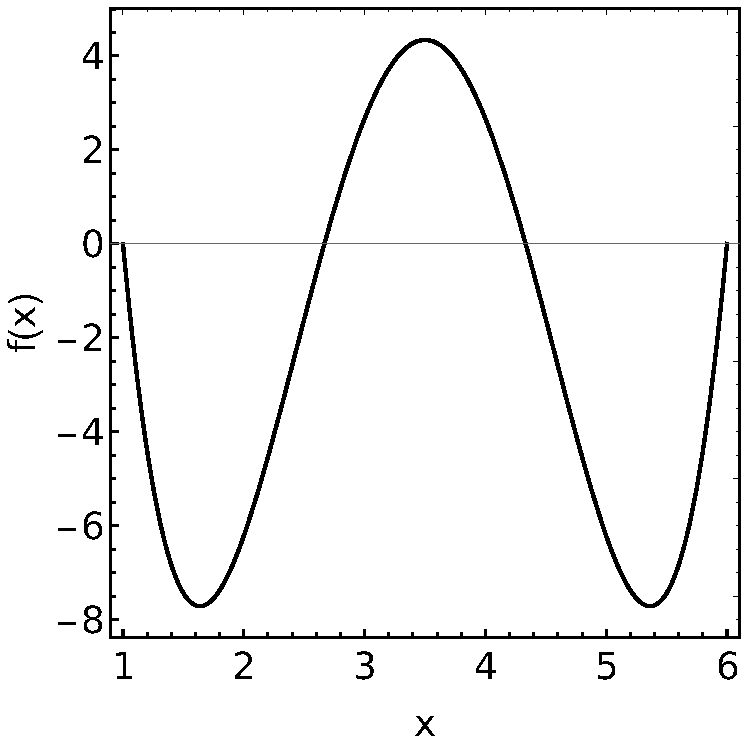
\includegraphics[width=1\linewidth]{task1_n3}} a) \\
\end{minipage}
\hfill
\begin{minipage}[h]{0.47\linewidth}
\center{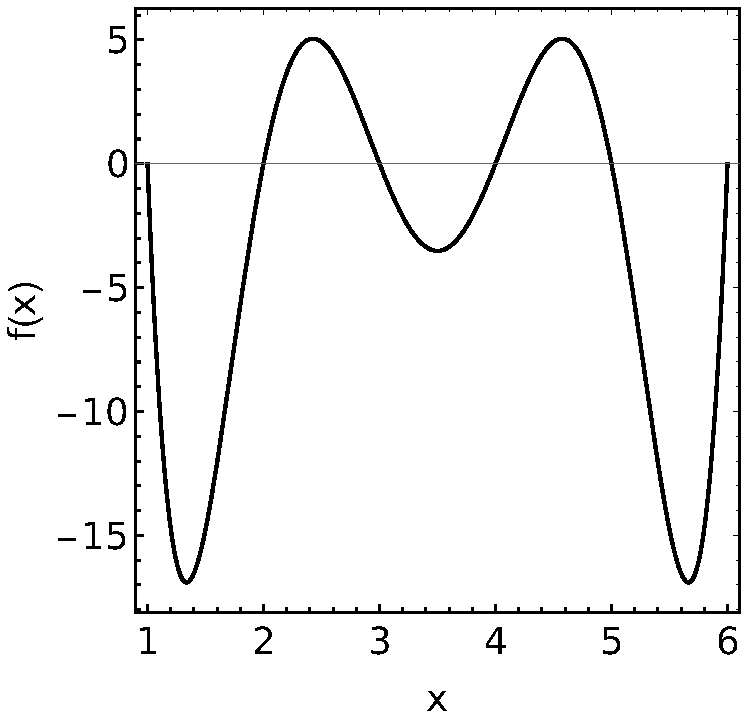
\includegraphics[width=1\linewidth]{task1_n5}} \\б)
\end{minipage}
\vfill
\begin{minipage}[h]{0.47\linewidth}
\center{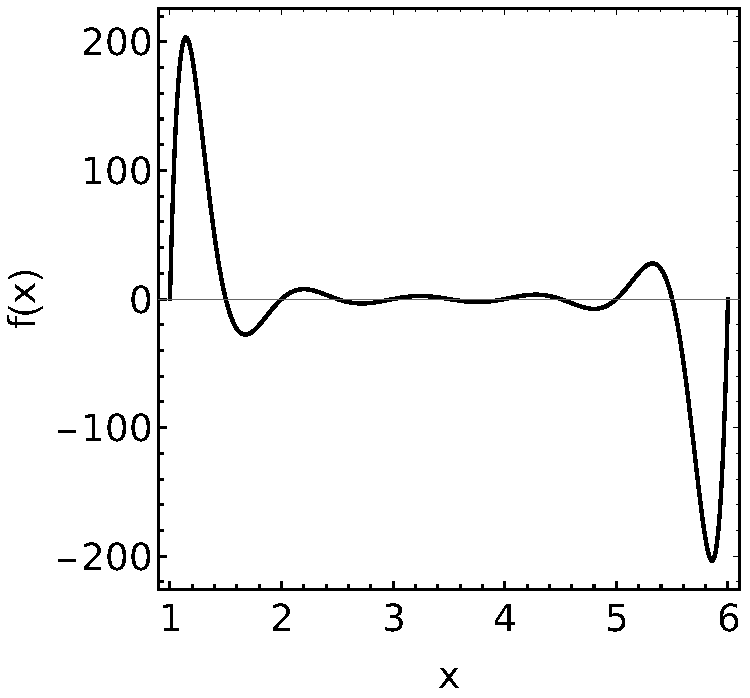
\includegraphics[width=1\linewidth]{task1_n10}} в) \\
\end{minipage}
\hfill
\begin{minipage}[h]{0.47\linewidth}
\center{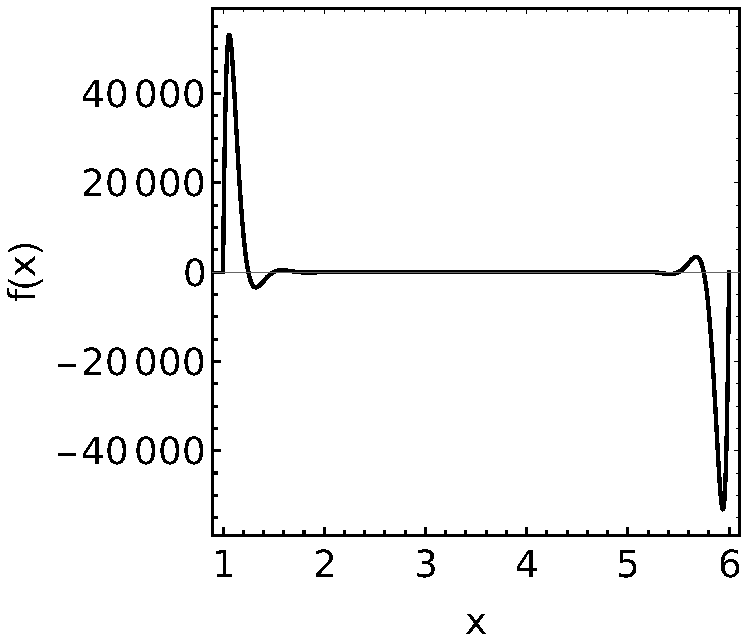
\includegraphics[width=1\linewidth]{task1_n20}} г) \\
\end{minipage}
\caption{Графики функции $\omega_{n+1}(x)$ для a) $n=3$, б) $n=5$, в) $n=10$, г) $n=20$.}
\label{ris:1}
\end{figure}

\newpage
\subsection*{Задание 2}
\begin{figure}[h]
\begin{minipage}[h]{0.47\linewidth}
\center{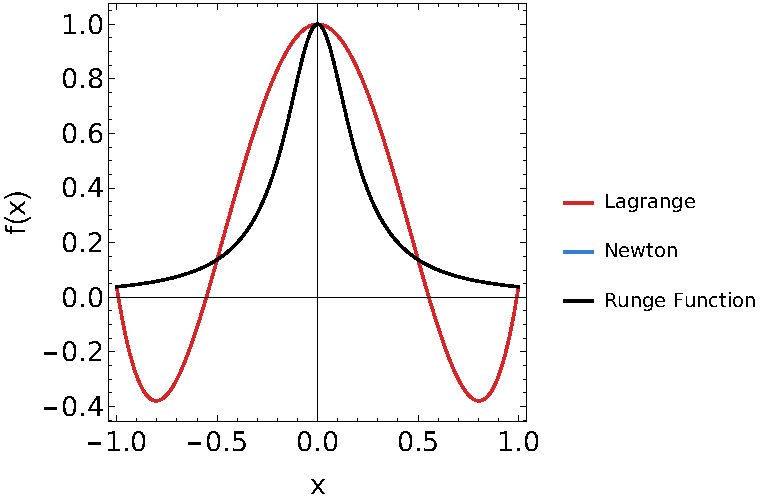
\includegraphics[width=1\linewidth]{task2_n5}} a) \\
\end{minipage}
\hfill
\begin{minipage}[h]{0.47\linewidth}
\center{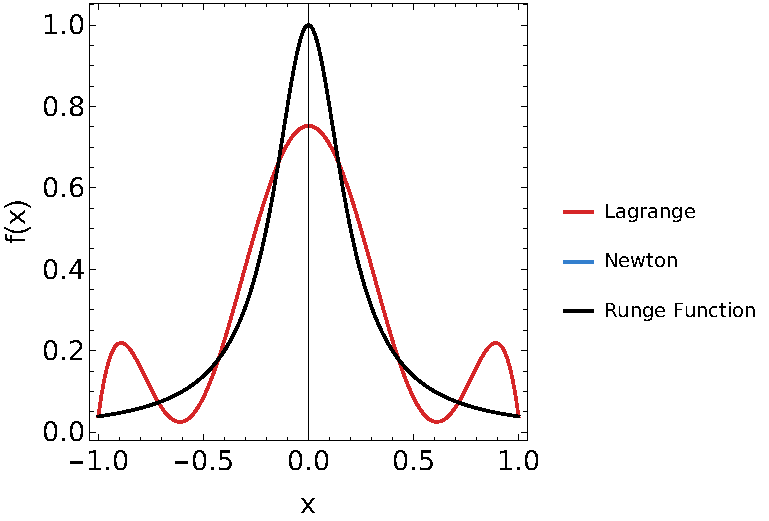
\includegraphics[width=1\linewidth]{task2_n8}} \\б)
\end{minipage}
\vfill
\begin{minipage}[h]{0.47\linewidth}
\center{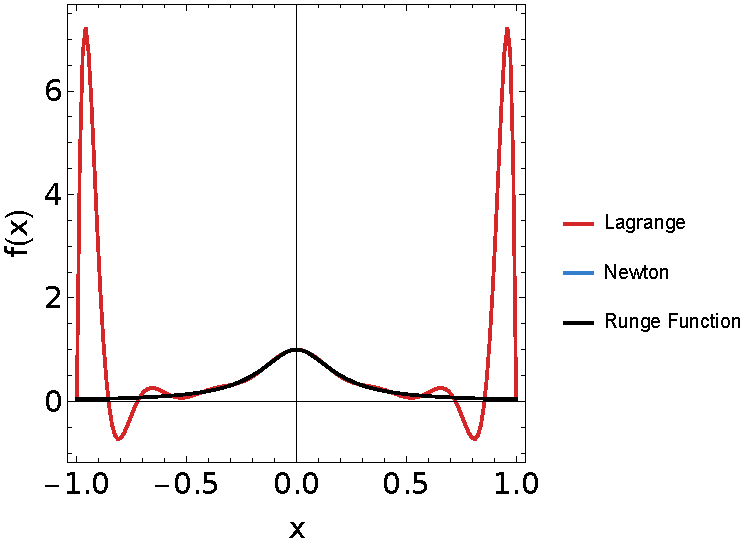
\includegraphics[width=1\linewidth]{task2_n15}} в) \\
\end{minipage}
\hfill
\begin{minipage}[h]{0.47\linewidth}
\center{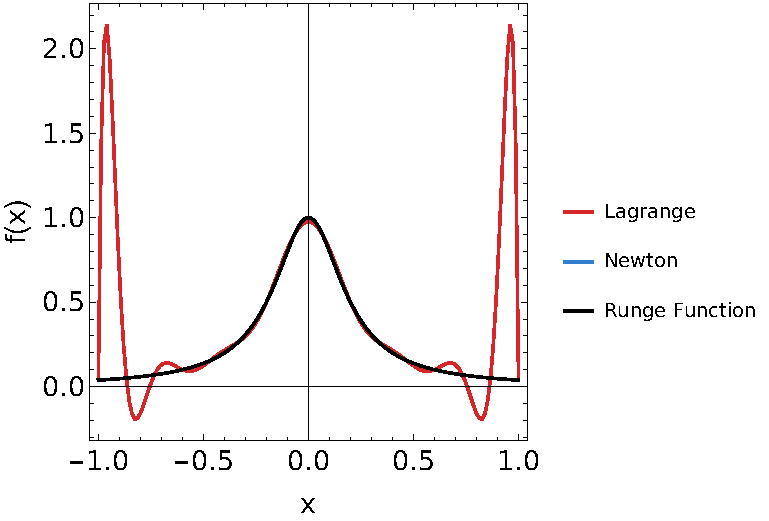
\includegraphics[width=1\linewidth]{task2_n16}} г) \\
\end{minipage}
\caption{Интерполяционные многочлены в форме Лагранжа и Ньютона, приближающие функцию Рунге для a) $n=5$, б) $n=8$, в) $n=15$, г) $n=16$.}
\label{ris:2}
\end{figure}

\section{Вывод}

Единственным способом улучшить оценку остаточного члена \\$\displaystyle|R_n(t)| = \left|\frac{f^{(n+1)}(\xi)}{(n+1)!}\omega_{n+1}(t)\right| \leq \frac{|f^{(n+1)}(\xi)|}{(n+1)!}\max_{[a,b]}{|\omega_{n+1}(t)|}$ в случае, если об интерполируемой функции известно только то, что она $n+1$ раз непрерывно дифференцируема, является выбор узлов сетки $\{t_i\}$ решением характерной задачи на минимакс:
$$\min_{t_0,t_1,...,t_n}\left[\max_{a\leq t\leq b}\left|\prod_{i=0}^n(t-t_i)\right|\right].$$
Из рассмотренных задач следует, что для максимума функции $|\omega_{n+1}(t)|$ наблюдается тенденция к увеличению значения при уменьшении шага разбиения равномерной сетки.


\end{document} 